\section{Uncertainties}\label{sec:unc}
\subsection{Statistical precision}
The numerator--denominator covariance must be retained when estimating efficiency errors. For data this requires a binomial construction where applicable; weighted simulation requires a treatment appropriate to its weights, including any negative weights. The supplied statistical and breakdown plots are retained without attributing an unverified interval algorithm to them.
\subsection{Topology, pileup and era dependence}
The supplied legends define jet-multiplicity regions $N_{\mathrm{jet}}<3$ and $N_{\mathrm{jet}}\geq3$, and vertex regions $N_{\mathrm{PV}}<40$ and $N_{\mathrm{PV}}\geq40$. These boundaries supersede the different provisional jet split in the original draft. The breakdown legends describe an envelope relative to the nominal SF. The intended interpretation is
\begin{equation}
\delta_k(i)=\max_{a\in\{\mathrm{low,high}\}}|\mathrm{SF}_{k,a}(i)-\mathrm{SF}_{\mathrm{nom}}(i)|,
\end{equation}
with relative uncertainty obtained by division by $|\mathrm{SF}_{\mathrm{nom}}(i)|$. This interpretation, including any statistical subtraction, must be checked against the production code. An era-dependence component is also shown; the plot alone does not specify its luminosity weighting or combination procedure.
\subsection{Reference--signal correlation}\label{sec:corr}
A useful diagnostic is
\begin{equation}
\alpha_c=\frac{P(R\cap S_c\mid O)}{P(R\mid O)P(S_c\mid O)},\qquad P(S_c\mid O,R)=\alpha_c P(S_c\mid O).
\end{equation}
Thus the reference-conditioned SF differs from the inclusive SF by $\alpha_d/\alpha_m$. An MC-only correlation study cannot determine this ratio in data without additional assumptions. The supplied orange curves are labelled as a correlation uncertainty, not as measurements of $\alpha$; they must not be relabelled as $\alpha$ distributions.
\subsection{Uncertainty combination and current limitation}
The supplied relative-breakdown legend defines total systematic uncertainty using era, jet multiplicity, and vertex multiplicity, and total uncertainty from statistics and that systematic term. Although a correlation curve is shown, it is absent from the stated systematic sum. This discrepancy requires resolution before adopting the total error or the accompanying 2D uncertainty maps. The draft reproduces the figures without changing their numerical content.
\subsubsection{2024 uncertainty breakdowns}
\begin{figure}[htbp]\centering
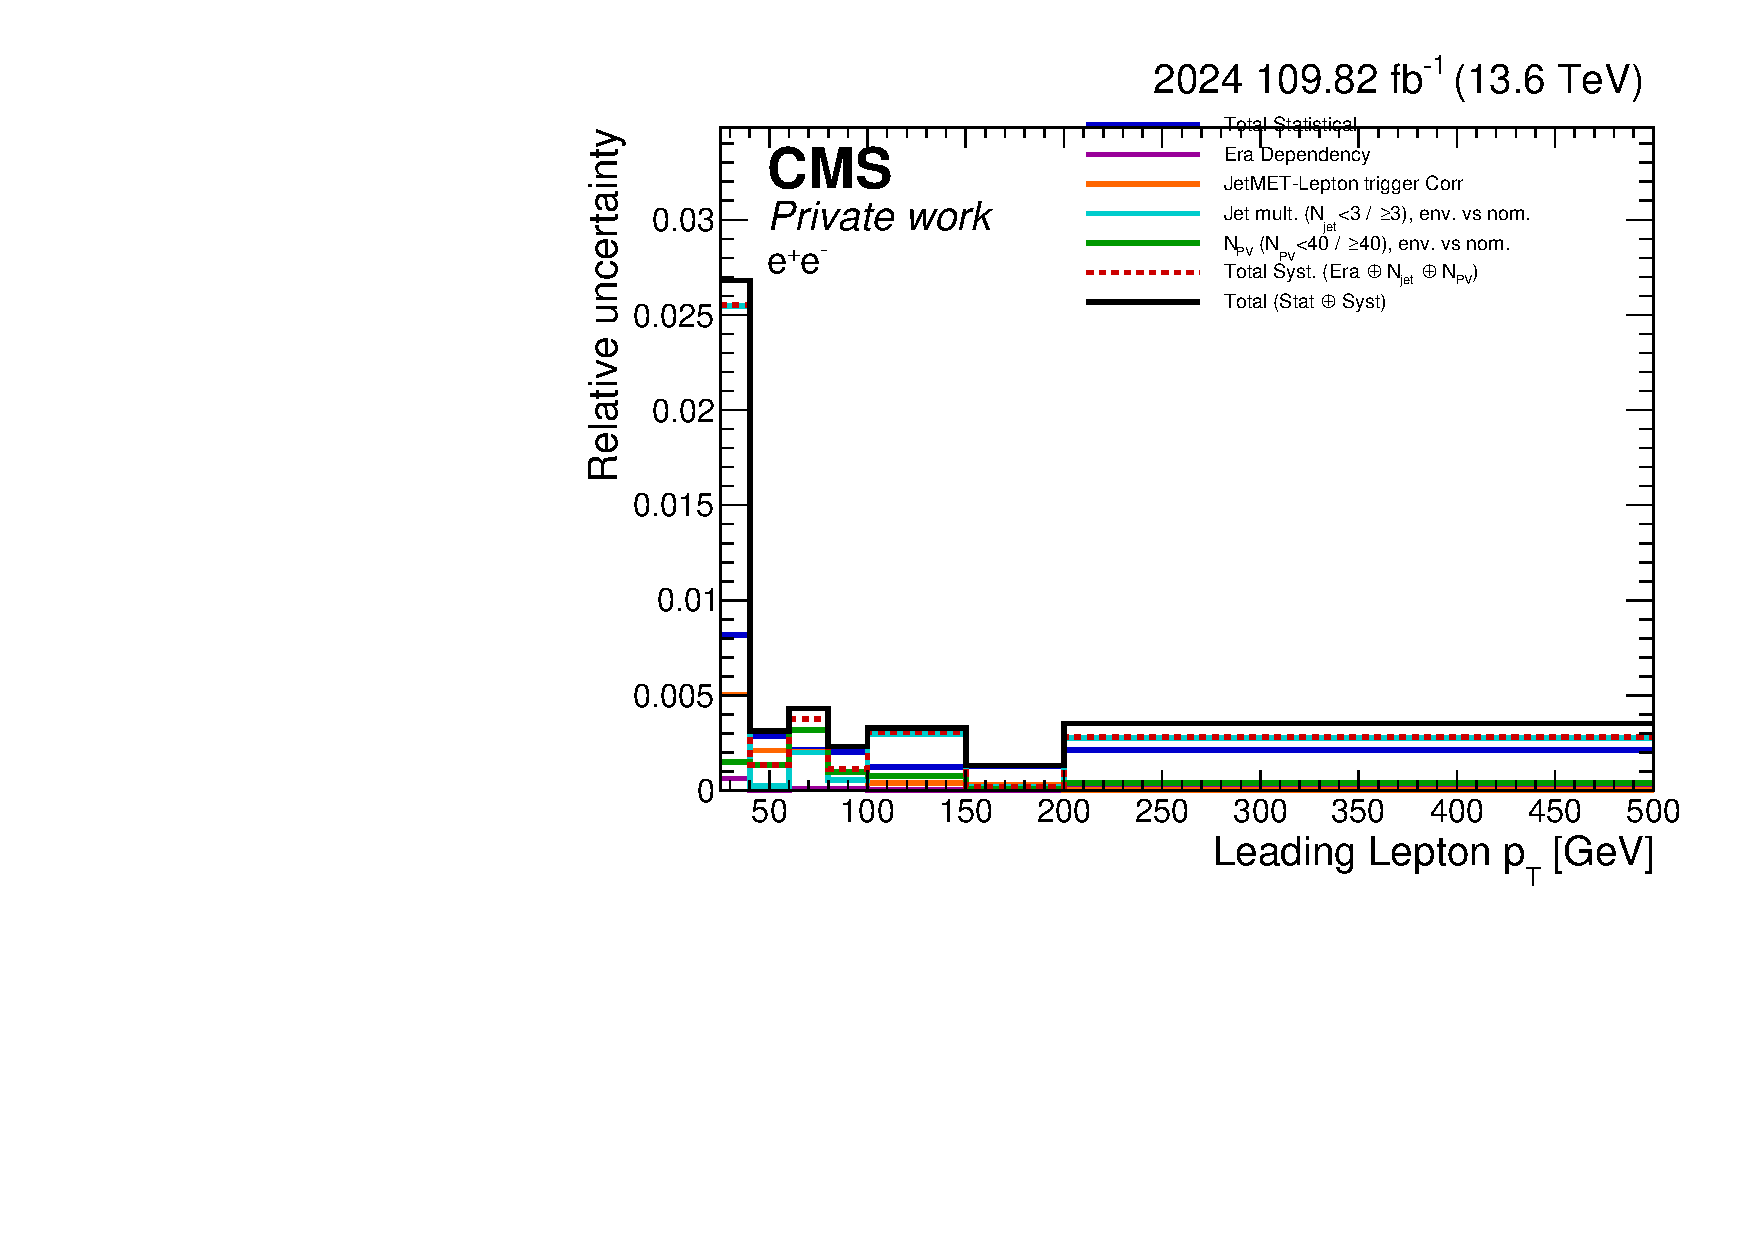
\includegraphics[width=0.48\linewidth]{figures/2024/ElEl/Relative_Uncertainty_Breakdown/Breakdown_Lep1pt.pdf}
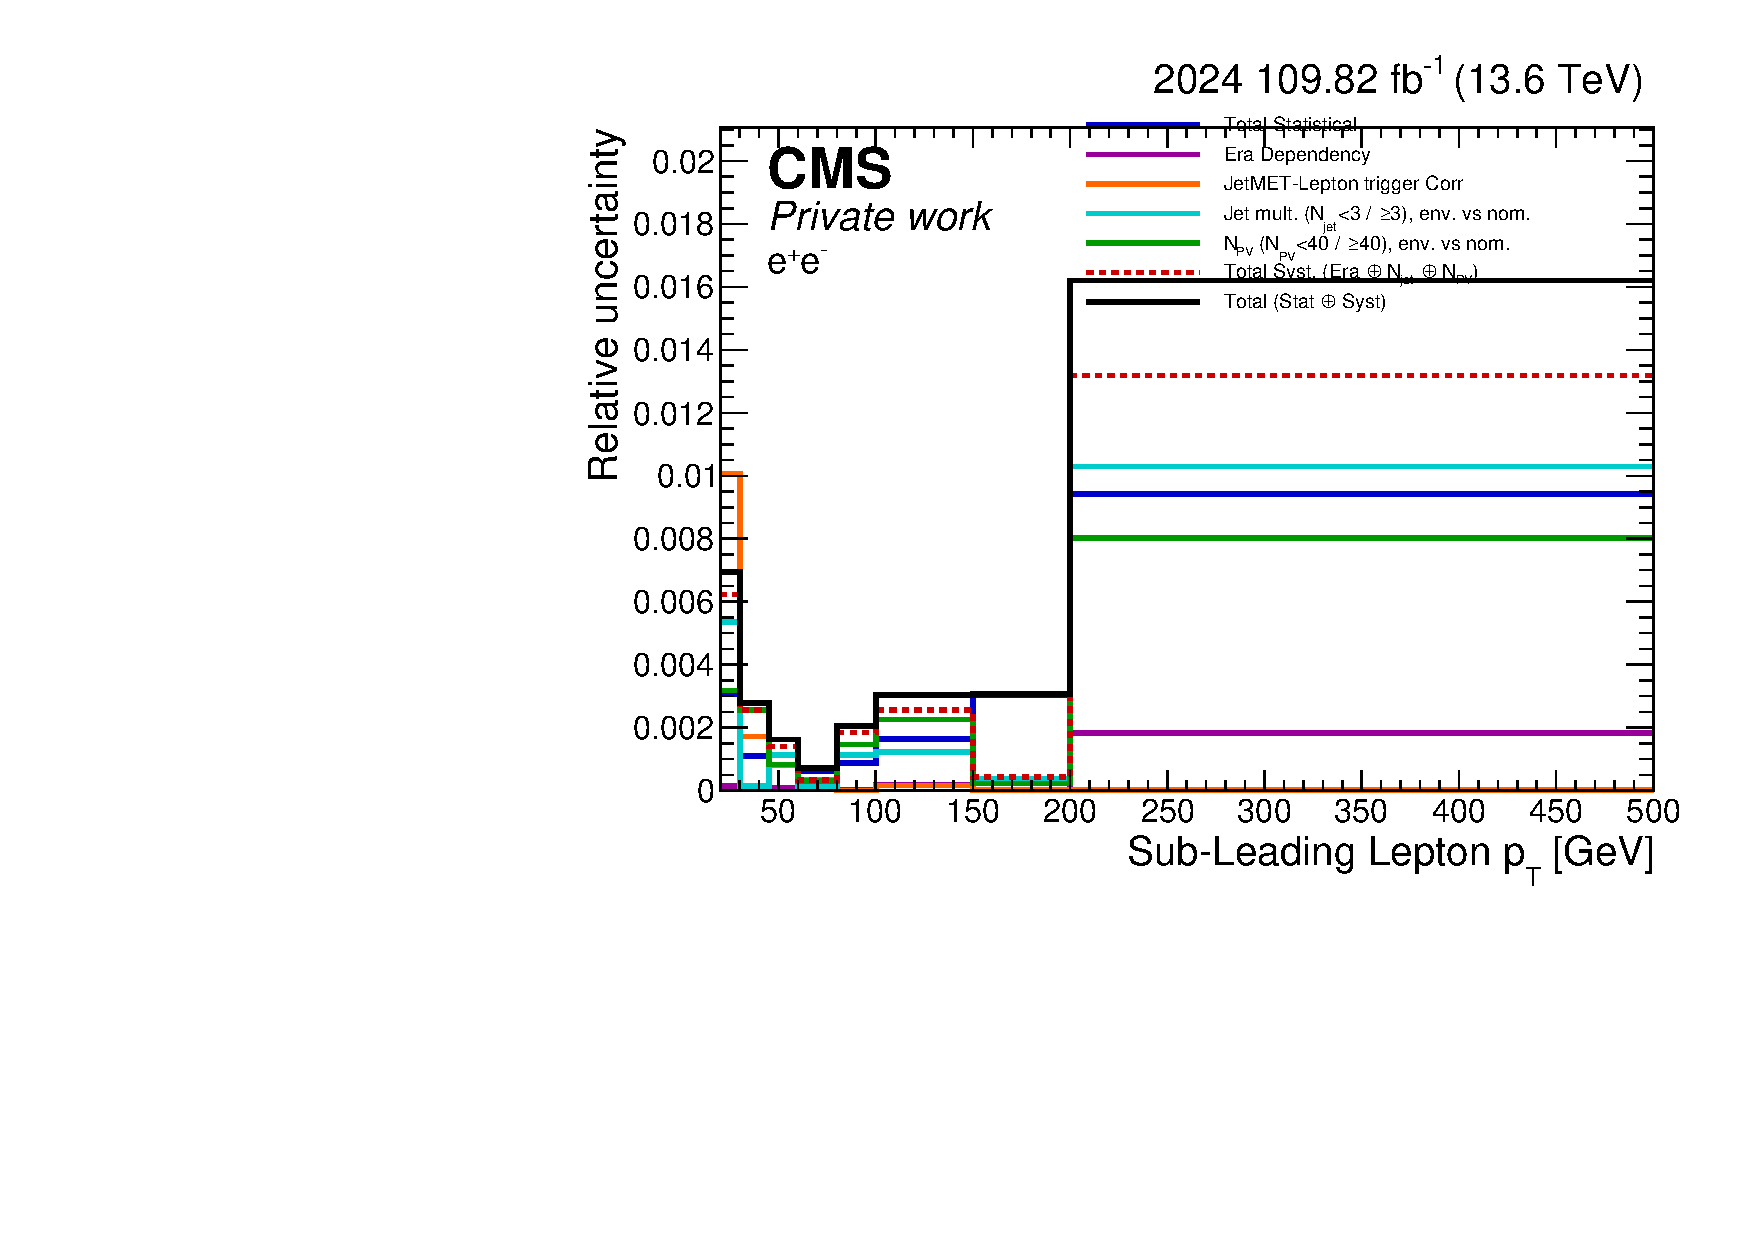
\includegraphics[width=0.48\linewidth]{figures/2024/ElEl/Relative_Uncertainty_Breakdown/Breakdown_Lep2pt.pdf}
\caption{2024: Relative uncertainty breakdown in the $ee$ channel versus leading and subleading lepton transverse momentum. The displayed total-systematic legend lists era, jet, and vertex components; the separately drawn correlation component is not listed in that sum.}\label{fig:unc-ElEl}
\end{figure}
\begin{figure}[htbp]\centering
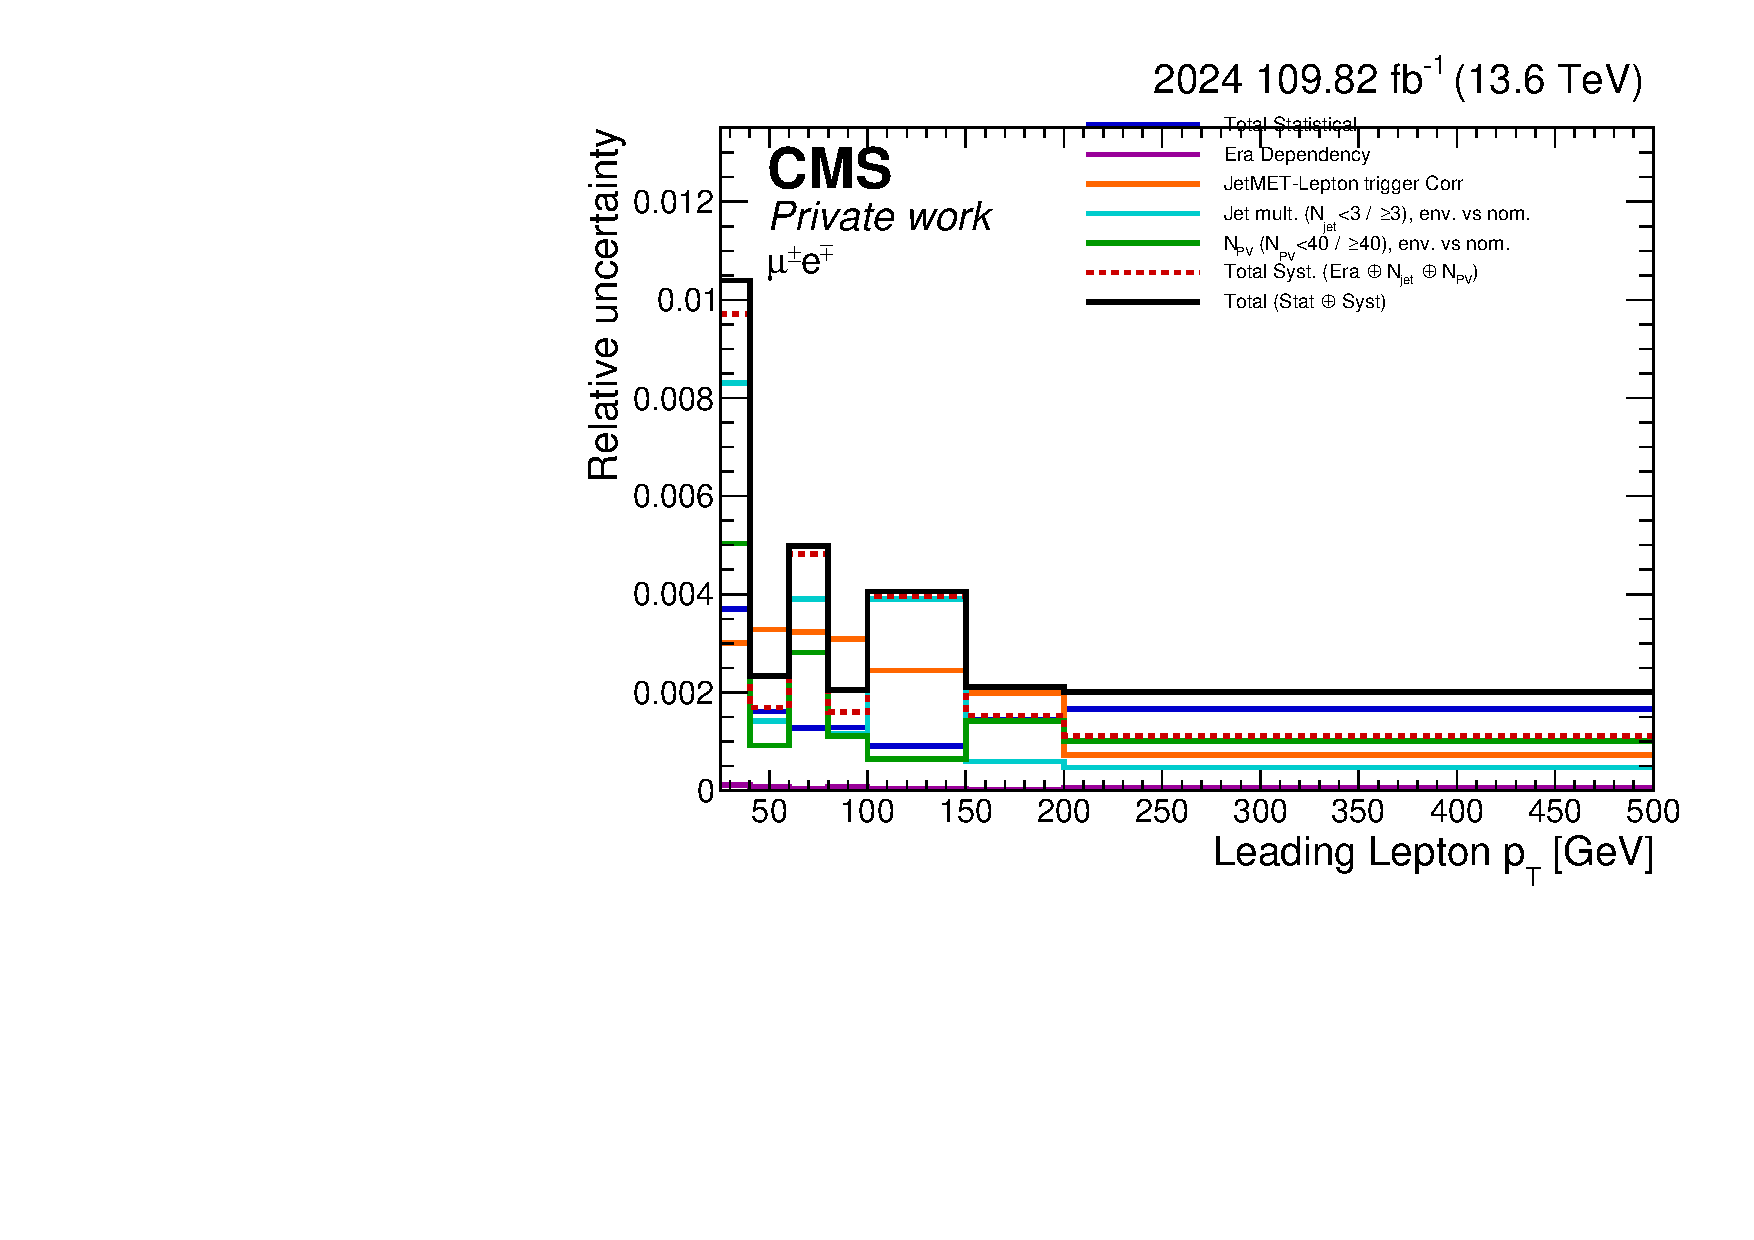
\includegraphics[width=0.48\linewidth]{figures/2024/MuEl/Relative_Uncertainty_Breakdown/Breakdown_Lep1pt.pdf}
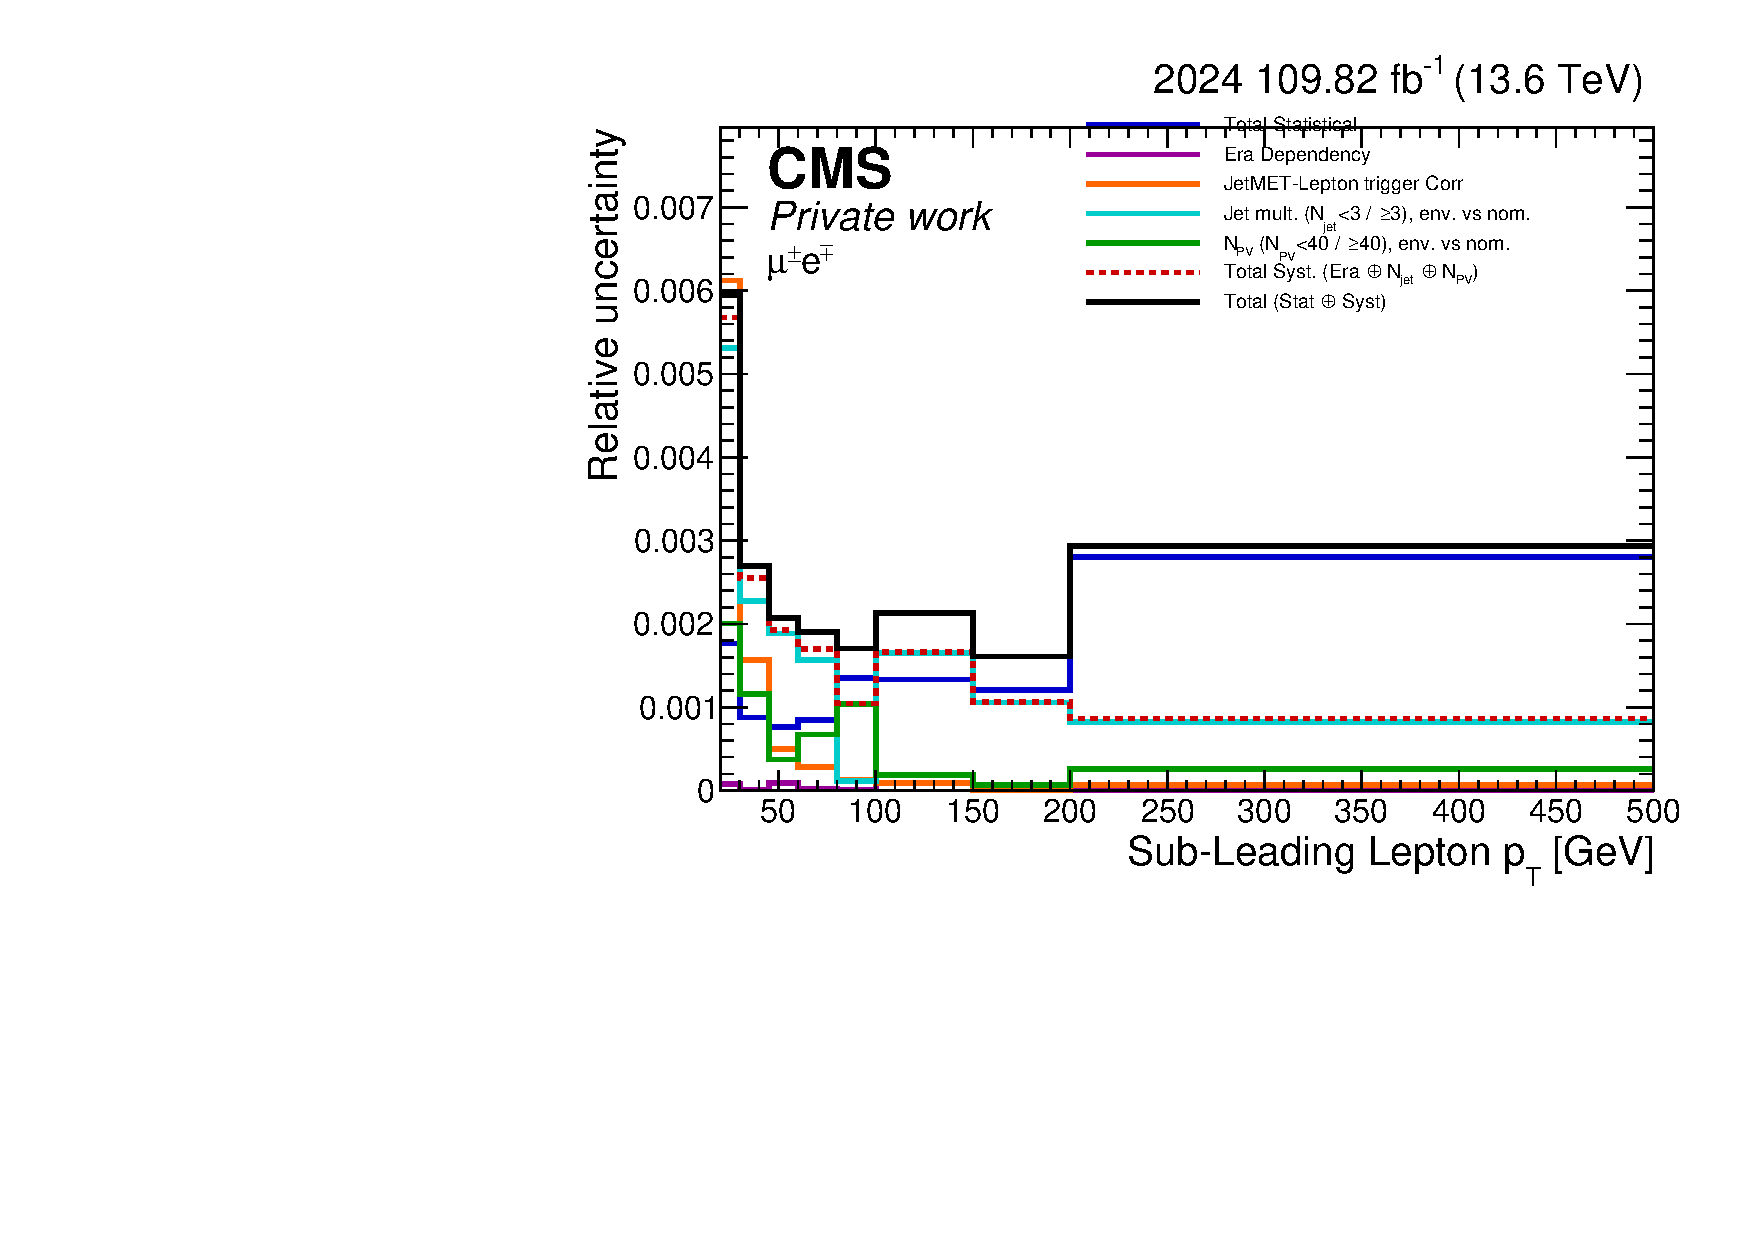
\includegraphics[width=0.48\linewidth]{figures/2024/MuEl/Relative_Uncertainty_Breakdown/Breakdown_Lep2pt.pdf}
\caption{2024: Relative uncertainty breakdown in the $e\mu$ channel versus leading and subleading lepton transverse momentum. The displayed total-systematic legend lists era, jet, and vertex components; the separately drawn correlation component is not listed in that sum.}\label{fig:unc-MuEl}
\end{figure}
\begin{figure}[htbp]\centering
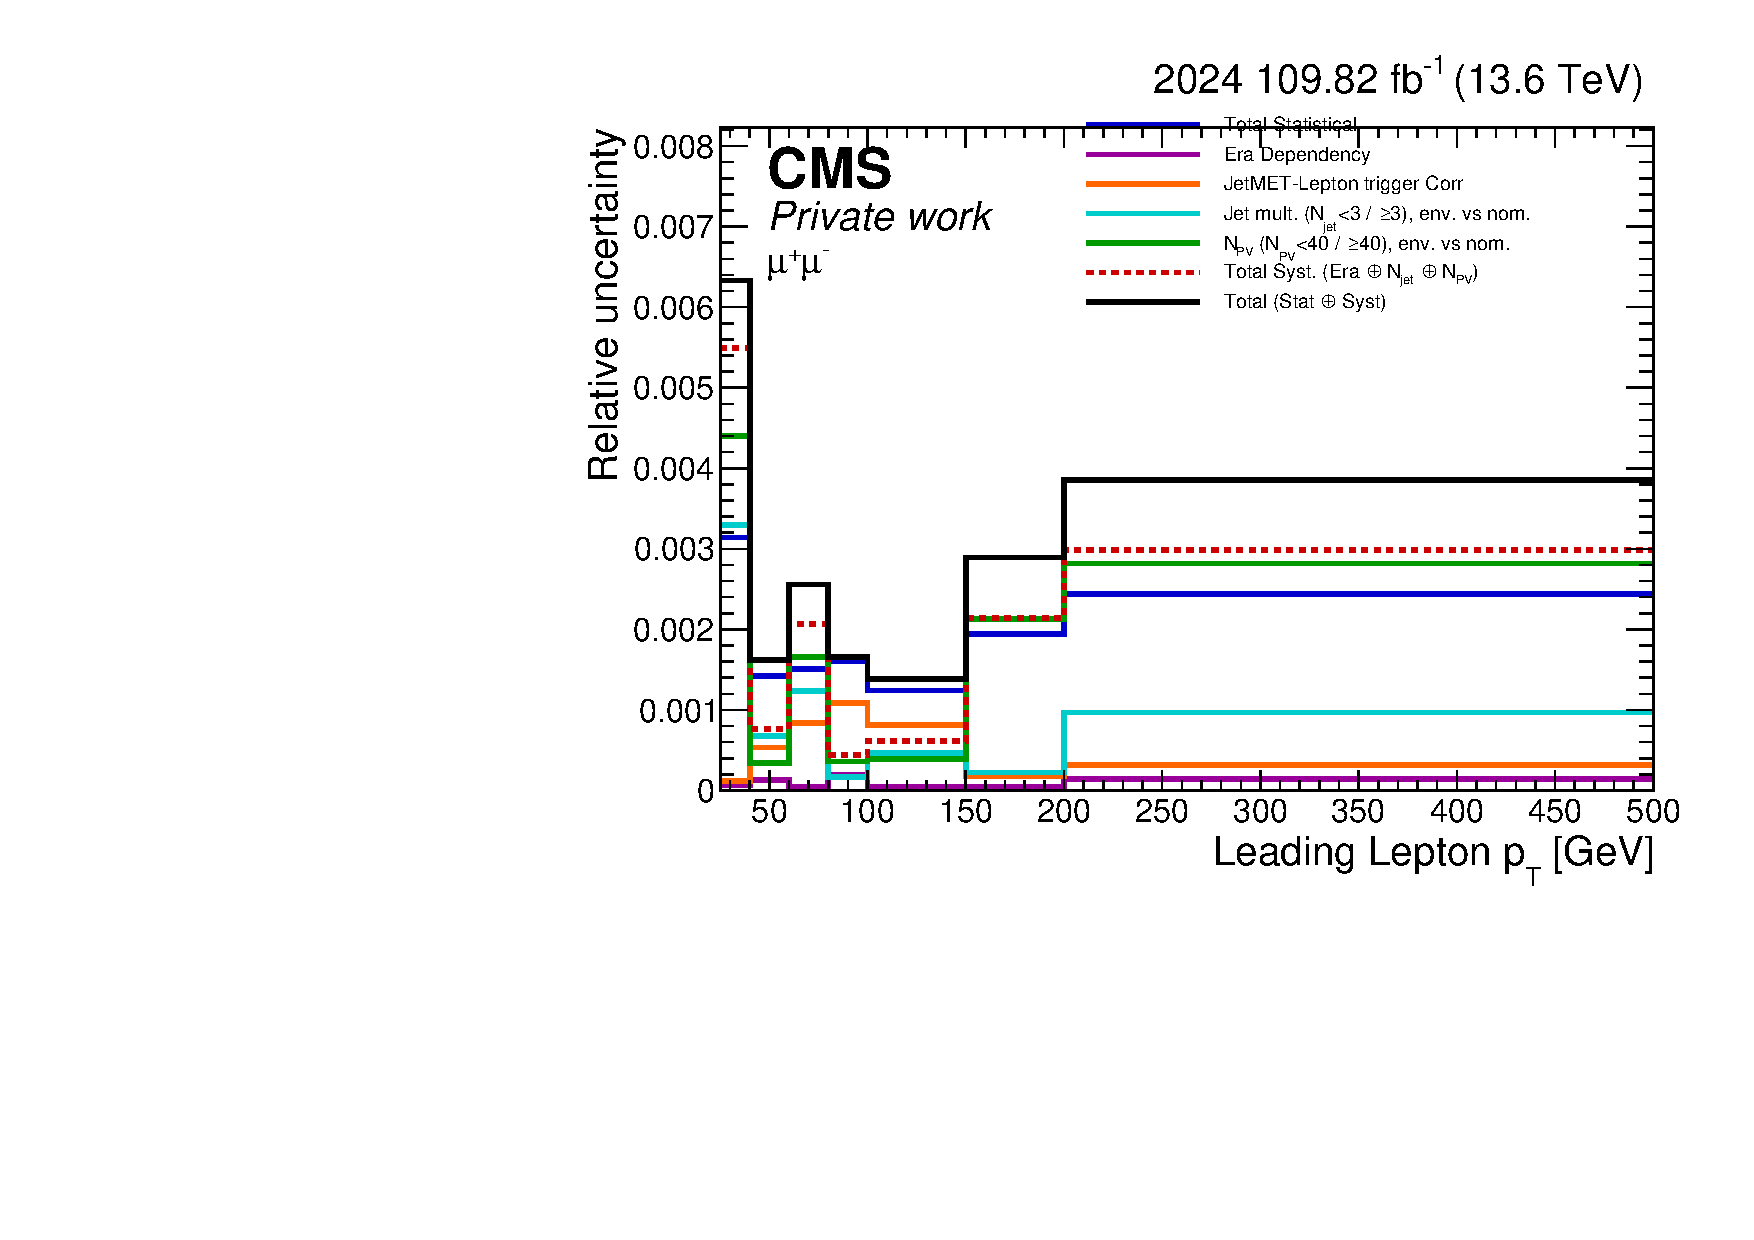
\includegraphics[width=0.48\linewidth]{figures/2024/MuMu/Relative_Uncertainty_Breakdown/Breakdown_Lep1pt.pdf}
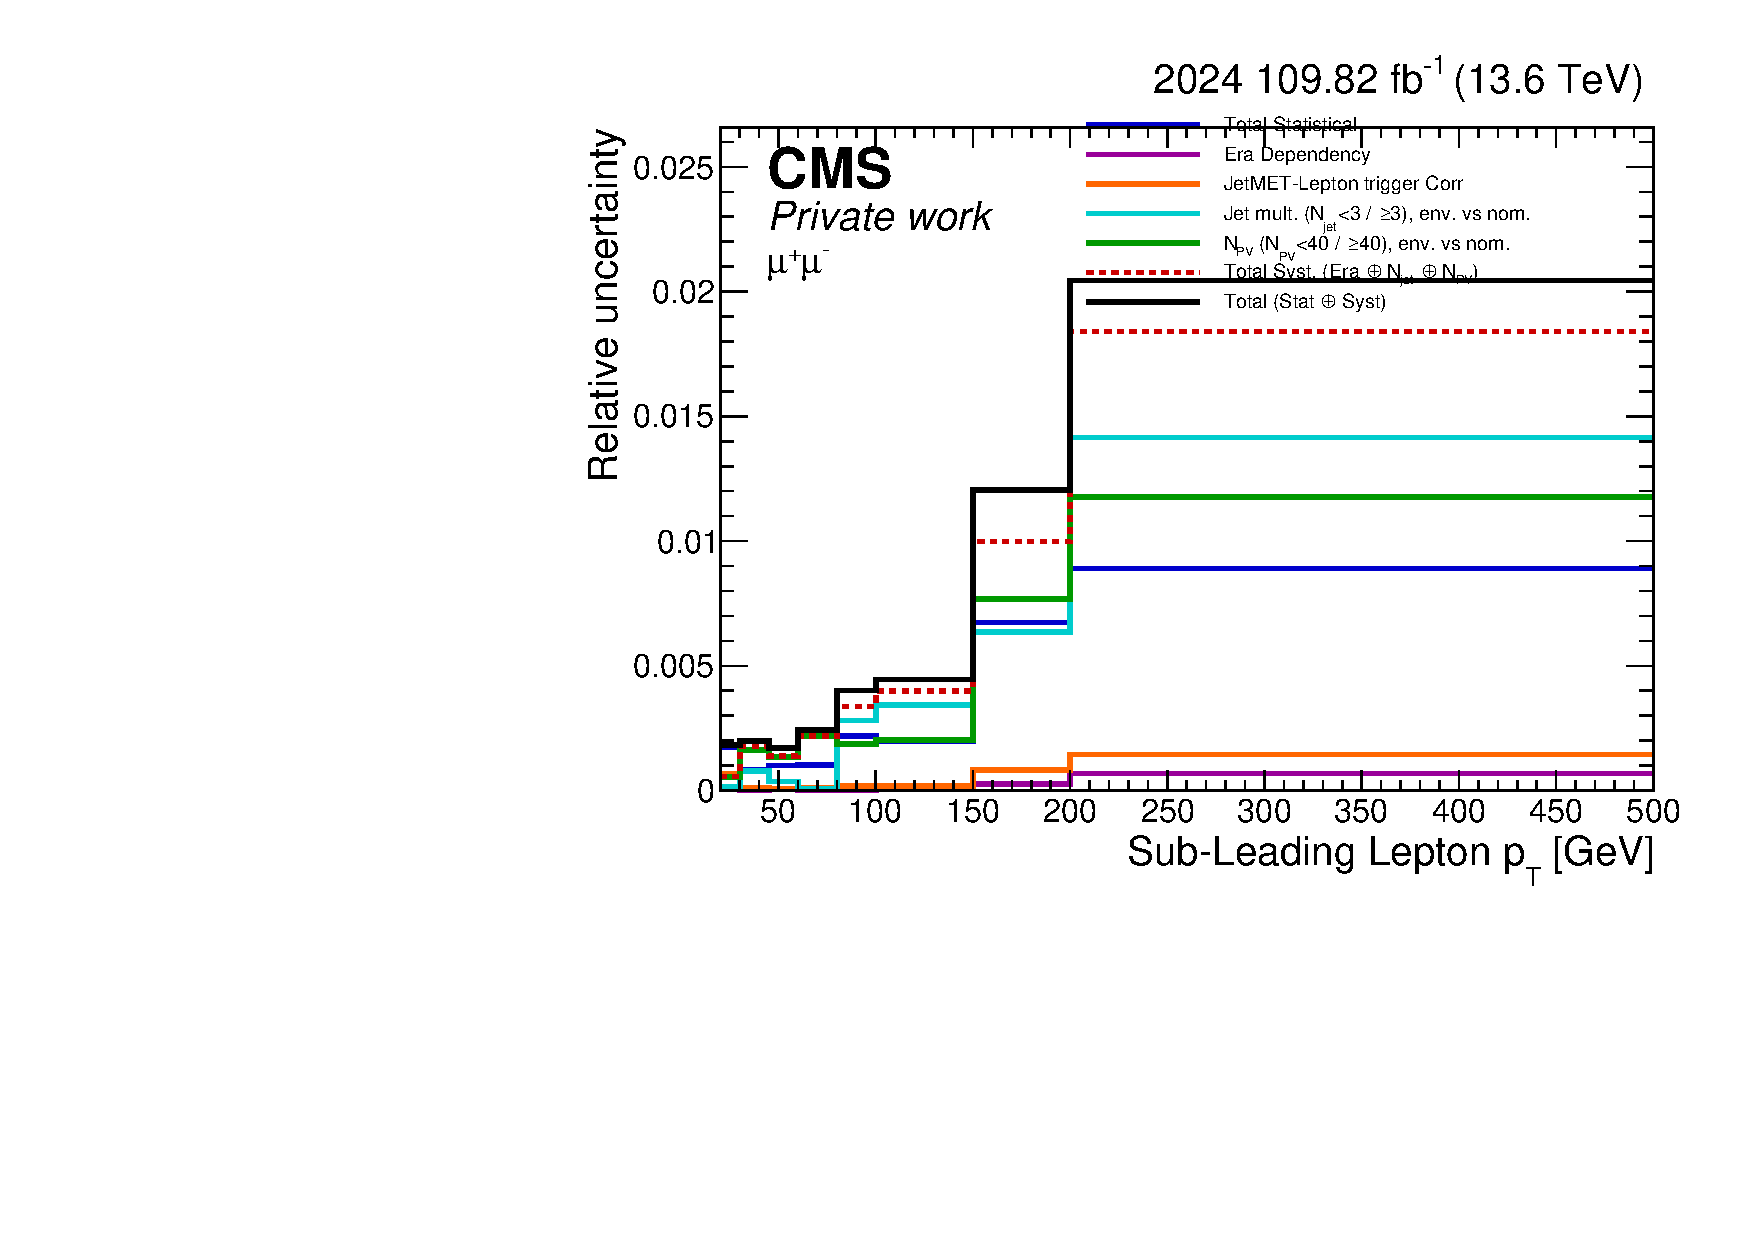
\includegraphics[width=0.48\linewidth]{figures/2024/MuMu/Relative_Uncertainty_Breakdown/Breakdown_Lep2pt.pdf}
\caption{2024: Relative uncertainty breakdown in the $\mu\mu$ channel versus leading and subleading lepton transverse momentum. The displayed total-systematic legend lists era, jet, and vertex components; the separately drawn correlation component is not listed in that sum.}\label{fig:unc-MuMu}
\end{figure}
\clearpage
\subsubsection{2025 uncertainty breakdowns}
\begin{figure}[htbp]\centering
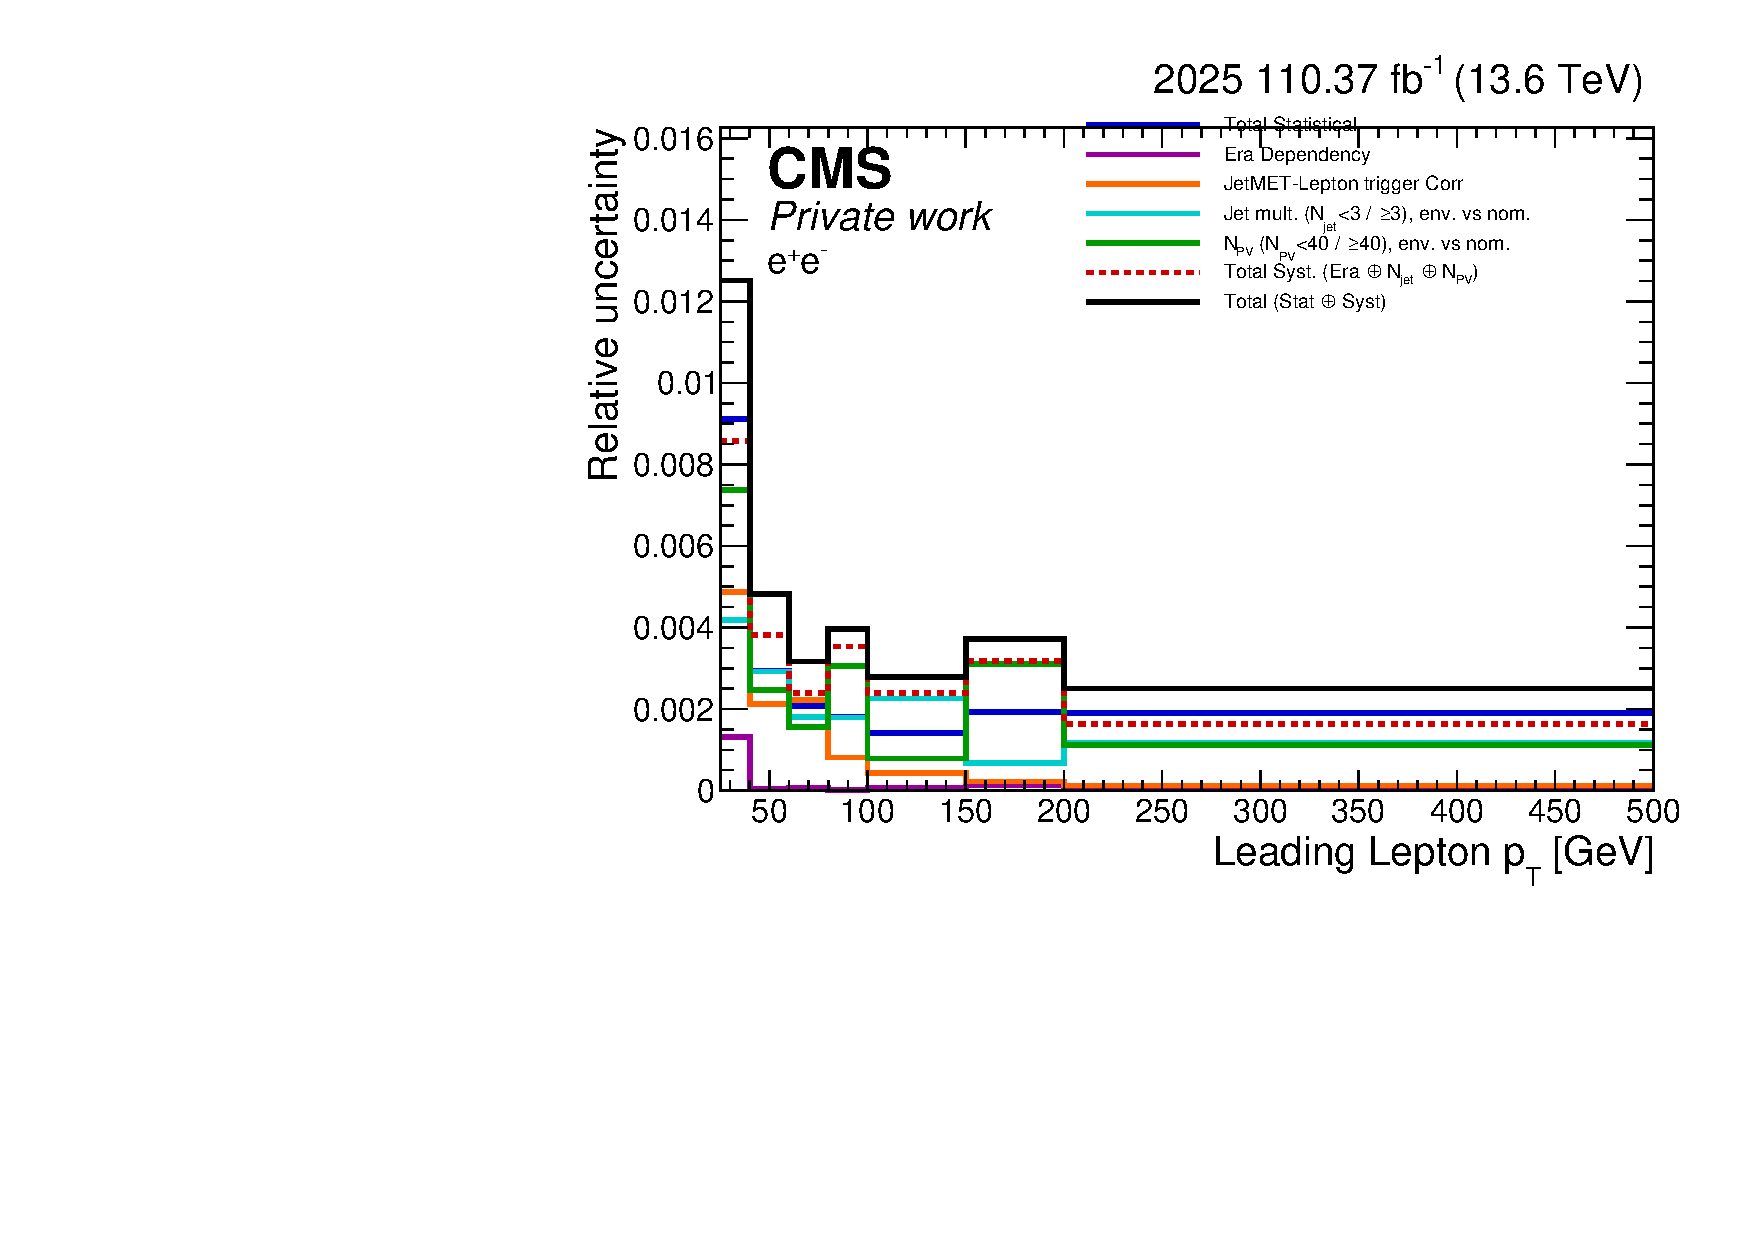
\includegraphics[width=0.48\linewidth]{figures/2025/ElEl/Relative_Uncertainty_Breakdown/Breakdown_Lep1pt.pdf}
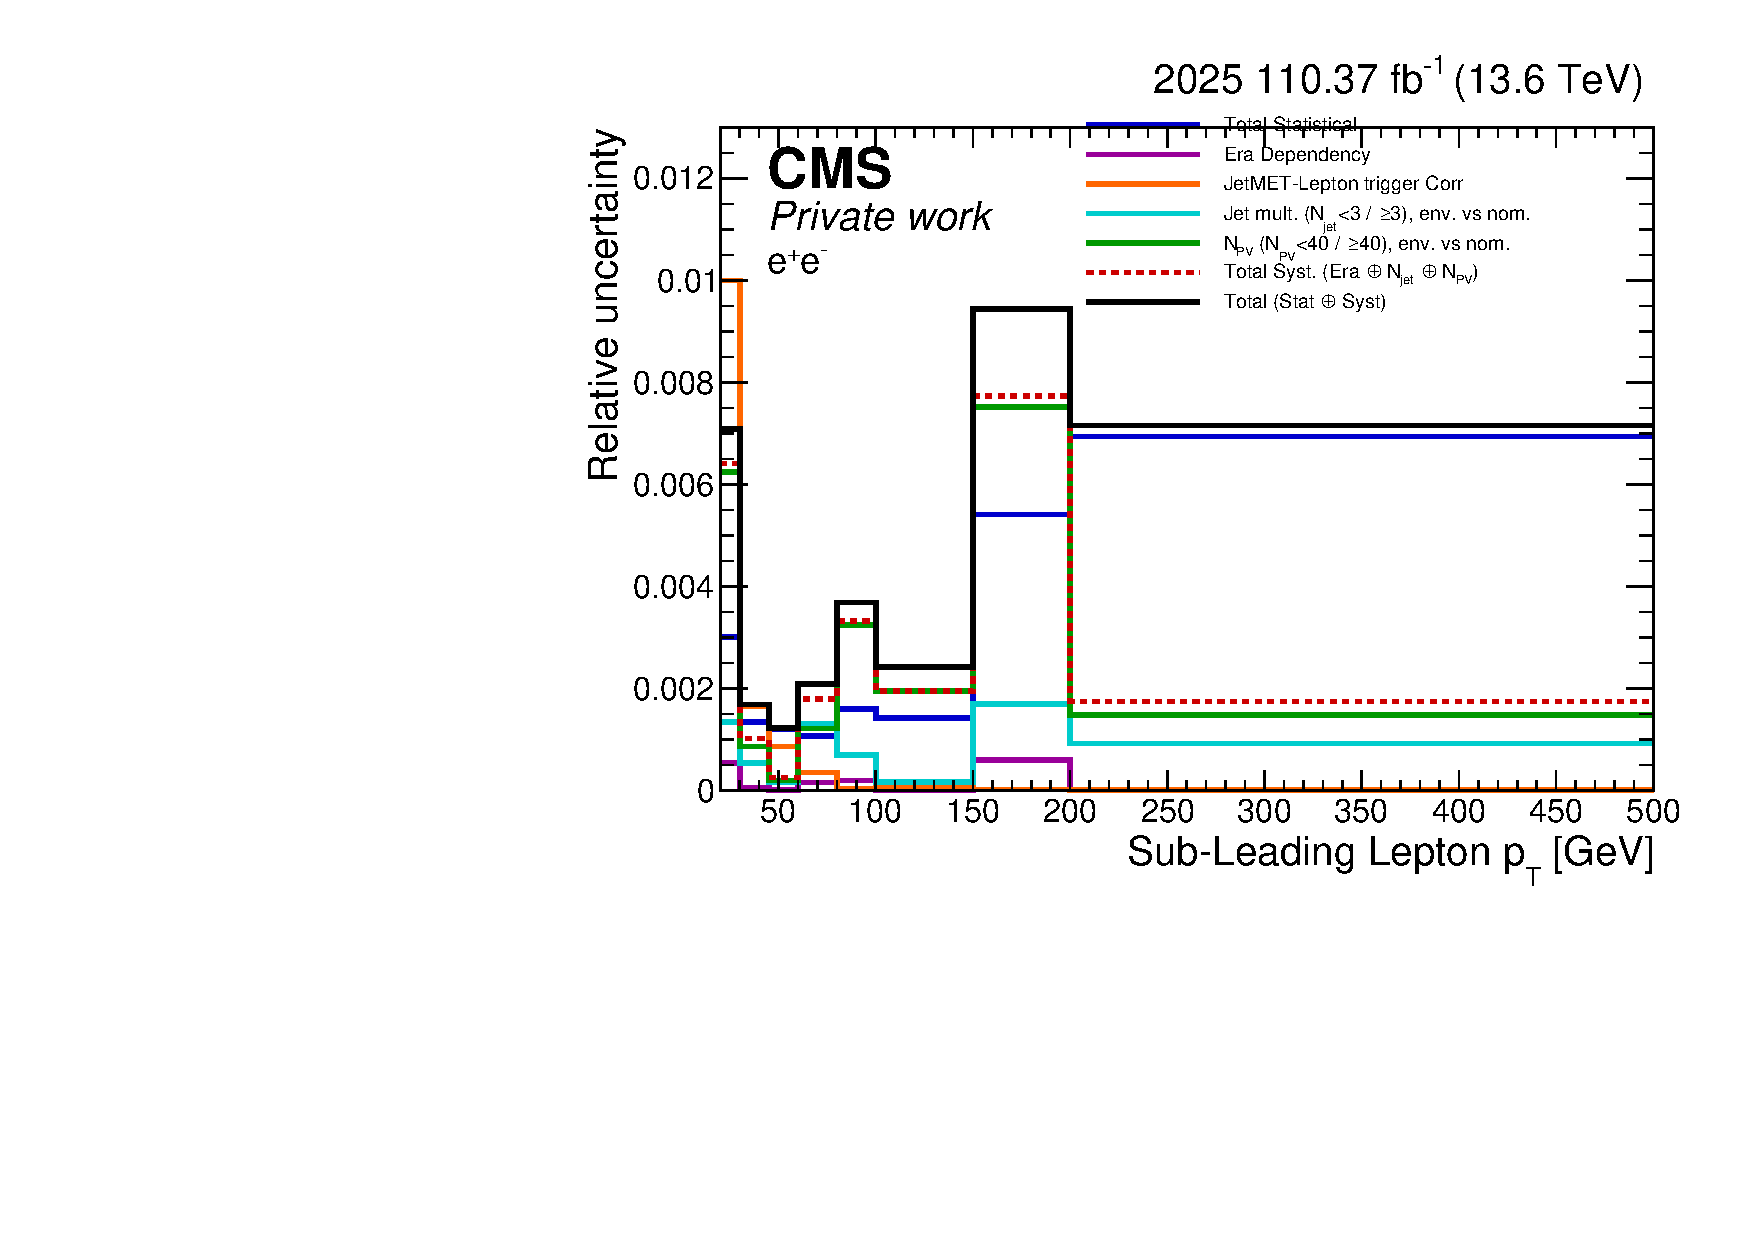
\includegraphics[width=0.48\linewidth]{figures/2025/ElEl/Relative_Uncertainty_Breakdown/Breakdown_Lep2pt.pdf}
\caption{2025: Relative uncertainty breakdown in the $ee$ channel versus leading and subleading lepton transverse momentum. The displayed total-systematic legend lists era, jet, and vertex components; the separately drawn correlation component is not listed in that sum.}\label{fig:unc-ElEl-2025}
\end{figure}
\begin{figure}[htbp]\centering
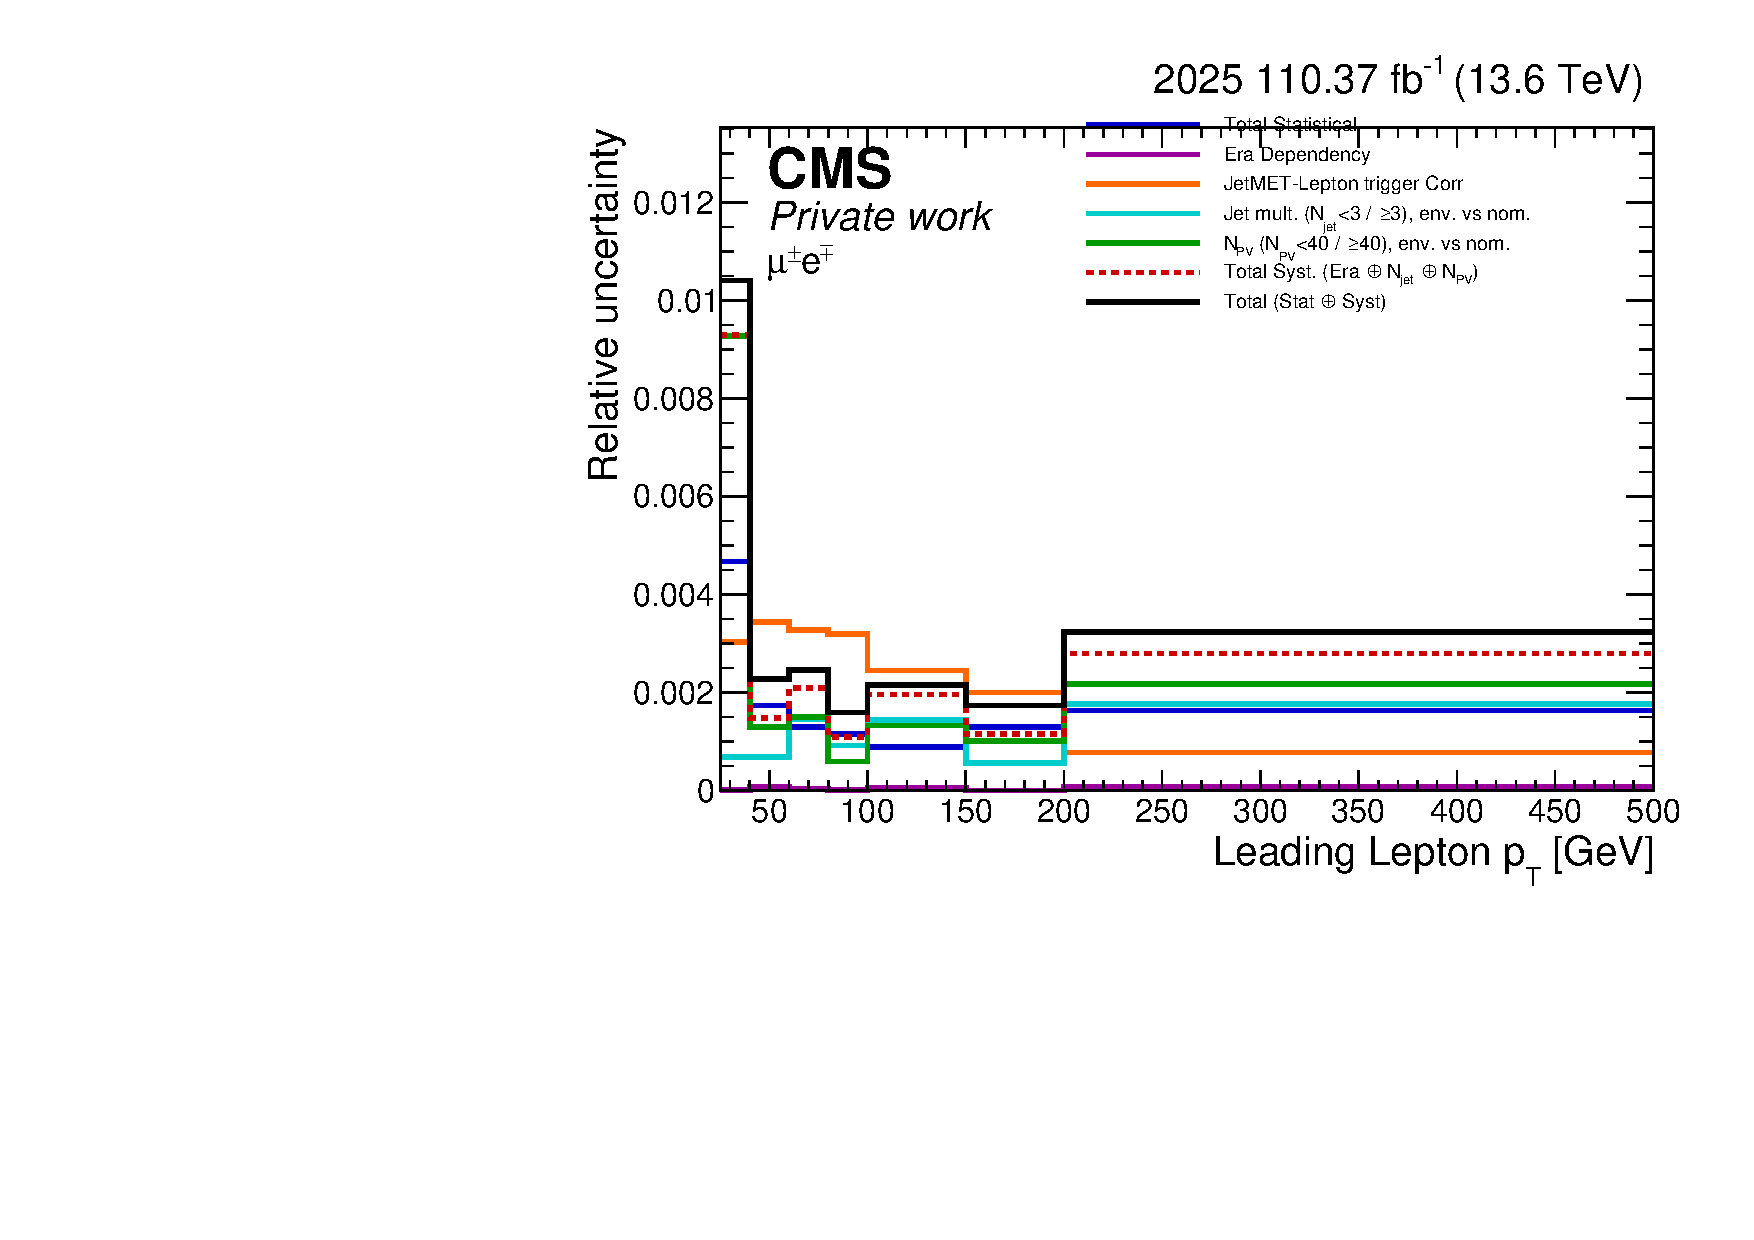
\includegraphics[width=0.48\linewidth]{figures/2025/MuEl/Relative_Uncertainty_Breakdown/Breakdown_Lep1pt.pdf}
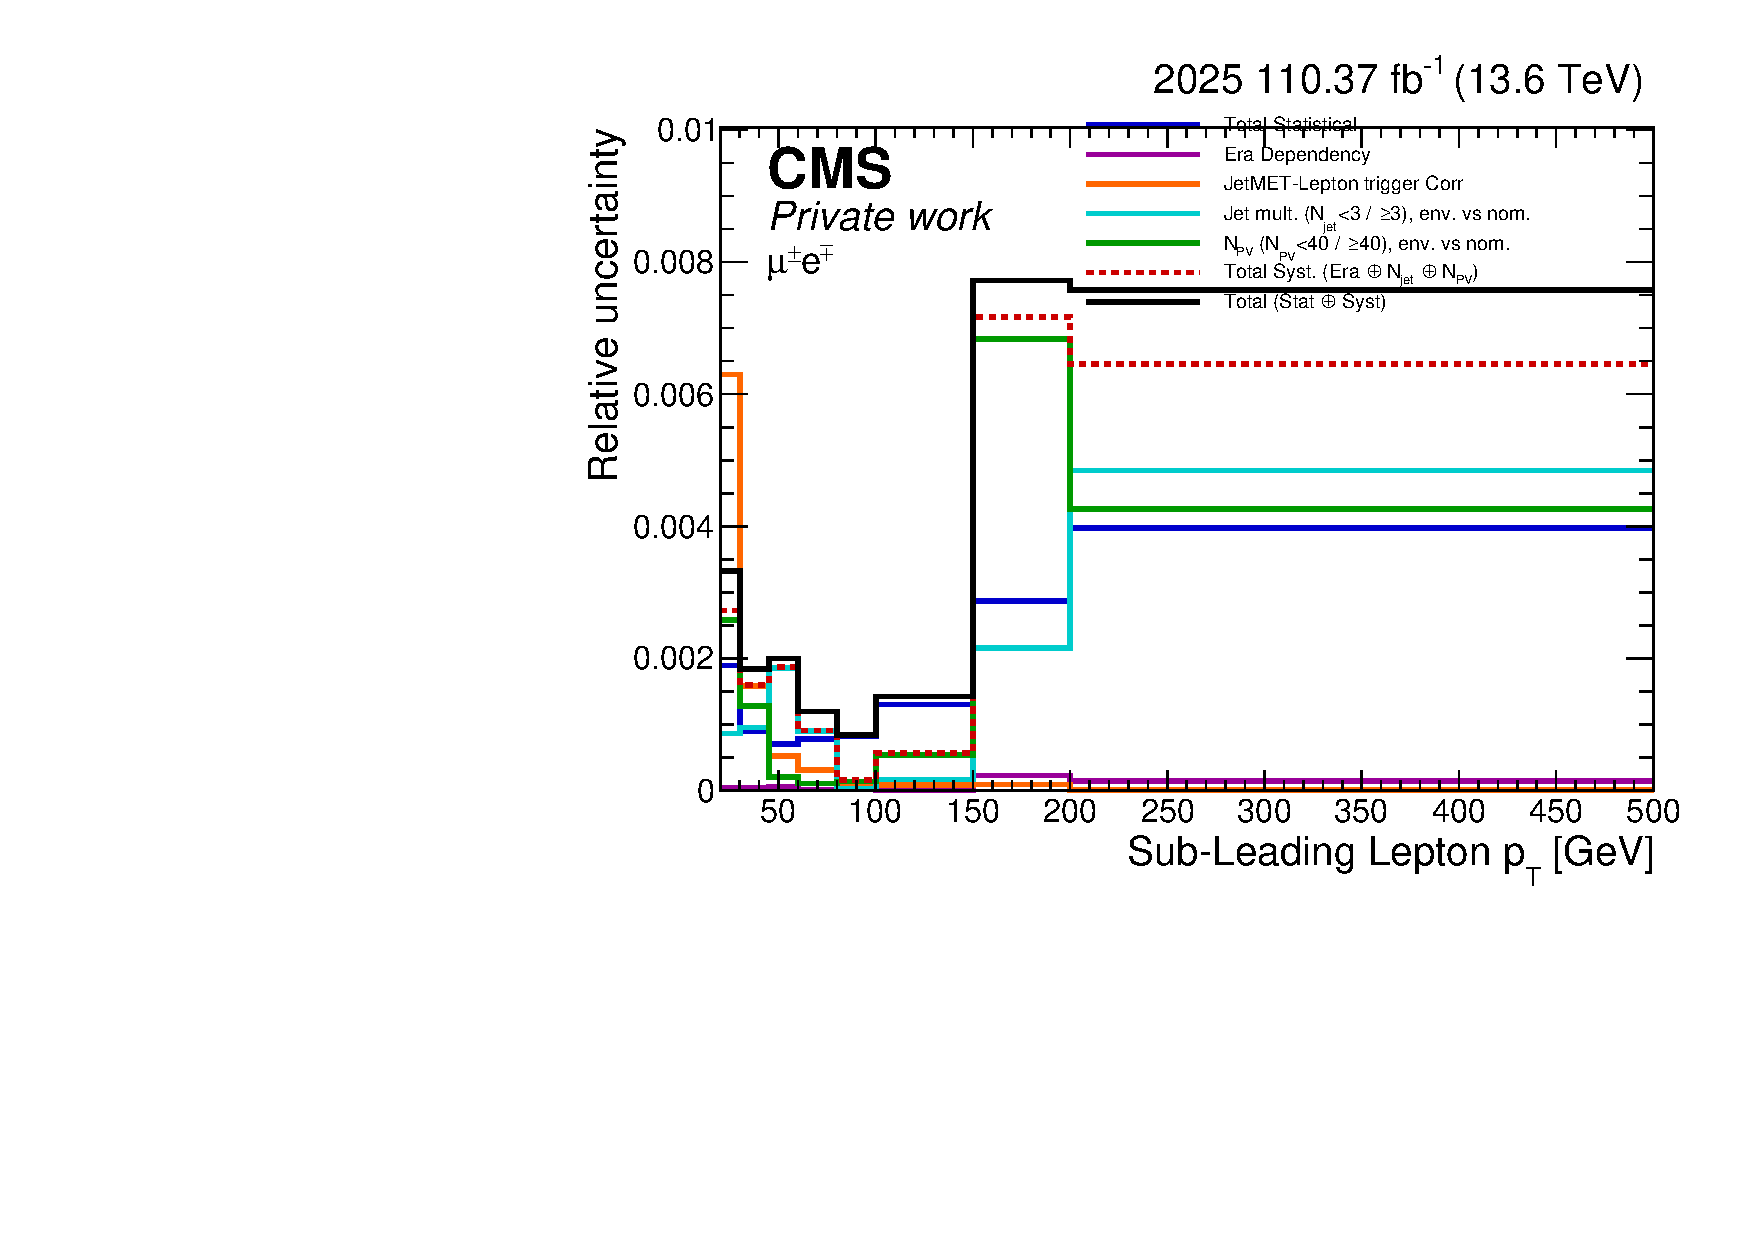
\includegraphics[width=0.48\linewidth]{figures/2025/MuEl/Relative_Uncertainty_Breakdown/Breakdown_Lep2pt.pdf}
\caption{2025: Relative uncertainty breakdown in the $e\mu$ channel versus leading and subleading lepton transverse momentum. The displayed total-systematic legend lists era, jet, and vertex components; the separately drawn correlation component is not listed in that sum.}\label{fig:unc-MuEl-2025}
\end{figure}
\begin{figure}[htbp]\centering
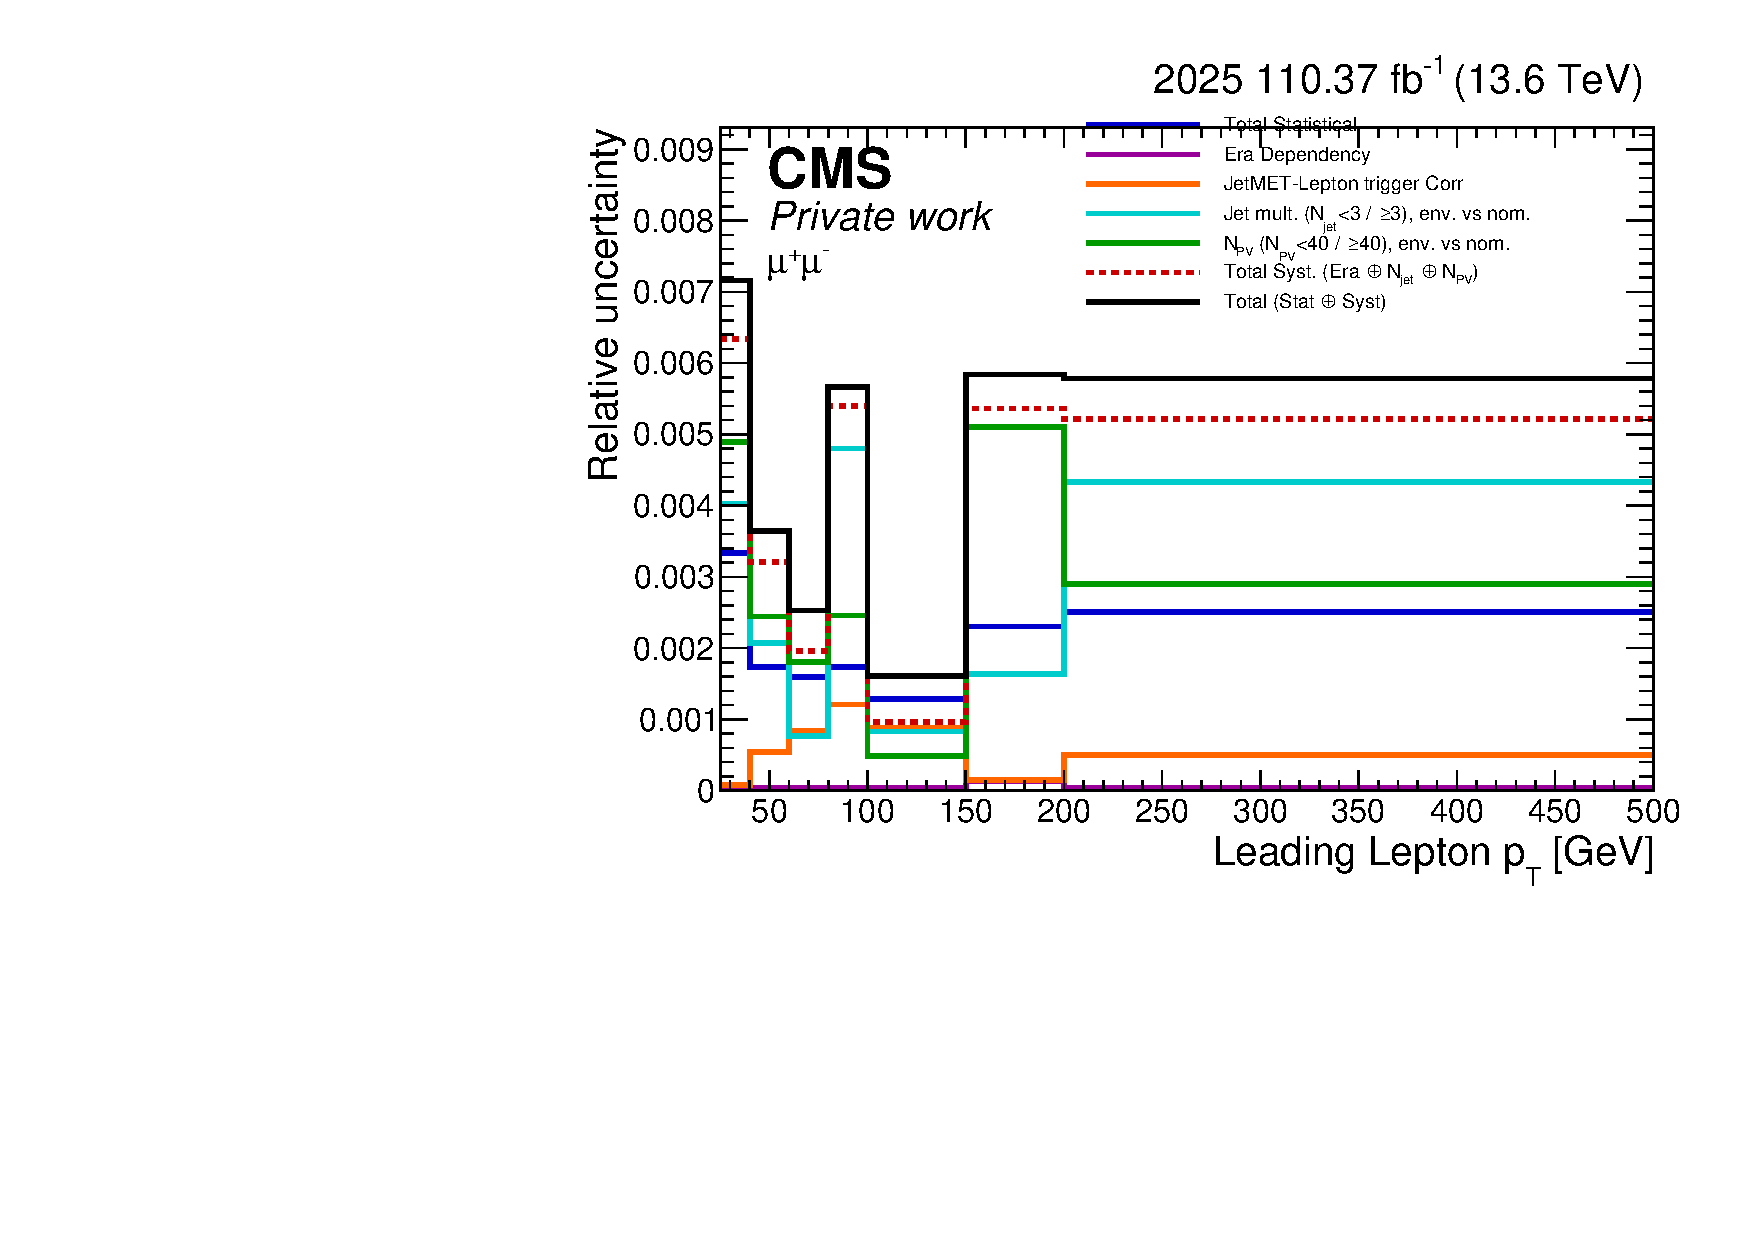
\includegraphics[width=0.48\linewidth]{figures/2025/MuMu/Relative_Uncertainty_Breakdown/Breakdown_Lep1pt.pdf}
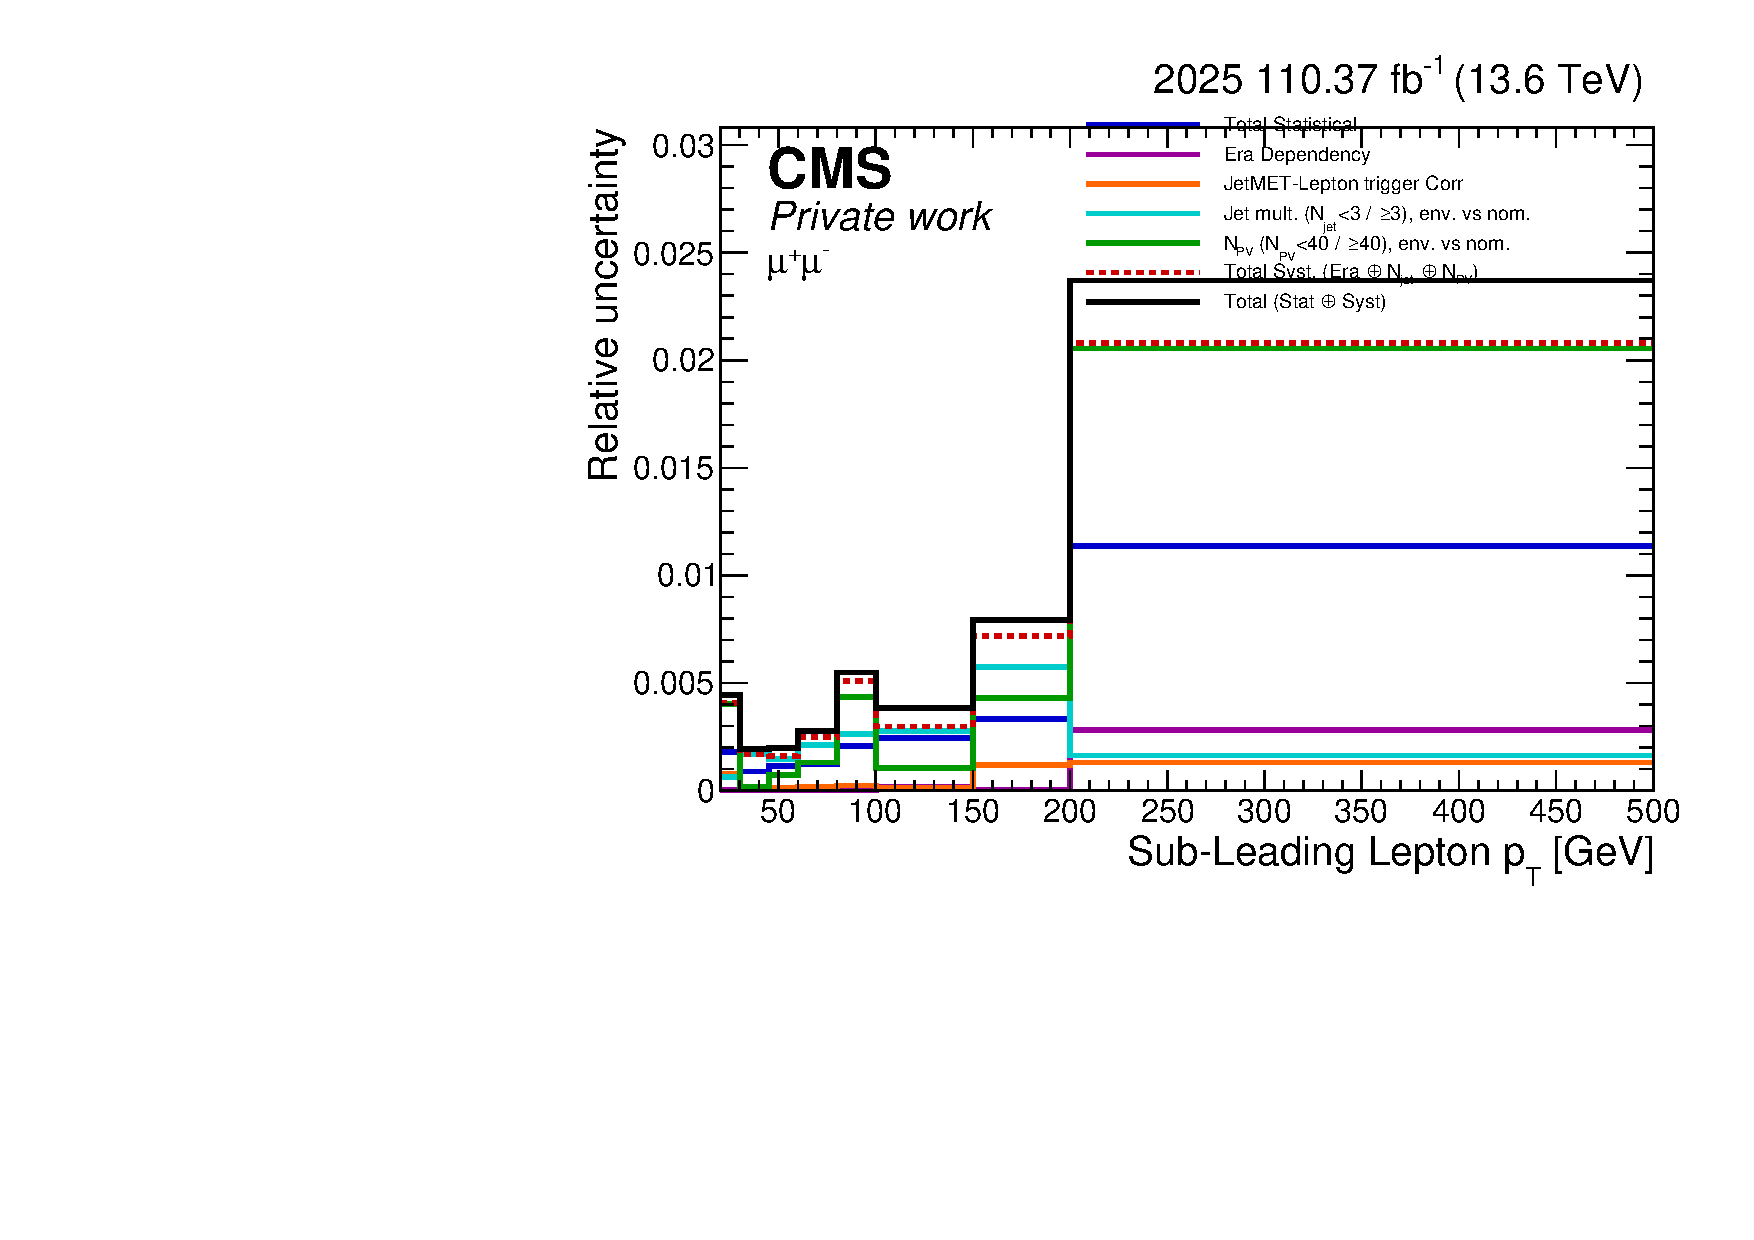
\includegraphics[width=0.48\linewidth]{figures/2025/MuMu/Relative_Uncertainty_Breakdown/Breakdown_Lep2pt.pdf}
\caption{2025: Relative uncertainty breakdown in the $\mu\mu$ channel versus leading and subleading lepton transverse momentum. The displayed total-systematic legend lists era, jet, and vertex components; the separately drawn correlation component is not listed in that sum.}\label{fig:unc-MuMu-2025}
\end{figure}
